\documentclass[num-refs]{wiley-article}
%\documentclass[times]{qjrms4}
%\documentclass[times,doublespace]{qjrms4}%For paper submission
\usepackage{color}
\usepackage[normalem]{ulem}  
\newcommand{\ma}[1]{\textcolor{blue}{#1}}  %comentarios Manuel 
\newcommand{\maxi}[1]{\textcolor{green}{#1}}  %comentarios Maxi 
\newcommand{\juan}[1]{\textcolor{magenta}{#1}}  %comentarios Juan 
\newcommand{\pierre}[1]{\textcolor{red}{#1}}  %comentarios Pierre 
\newcommand{\me}[1]{\sout{#1}}  
\usepackage{amsfonts} % added for mathbb

% from Trang
\usepackage{multirow}
\usepackage[scr=esstix,cal=boondox]{mathalfa} 
\usepackage{hyperref}
\hypersetup{
    colorlinks=true,
    urlcolor=black,
    citecolor=blue,
}
\usepackage[ruled,vlined]{algorithm2e} 


% From Pierre T.
\renewcommand{\v}[1]{\ensuremath{\mathbf{#1}}}
\newcommand{\gv}[1]{\bm{#1}}
\newcommand{\transp}{\mathrm{T}}
\usepackage[nice]{nicefrac}

% Update article type if known
\papertype{Research Article}


\begin{document}
\runningauthor{Sacco M. A. et al. }
%\runningheads{Sacco M. A. et al. }{ML uncertainty quantification for DA}

\title{Online machine-learning forecast uncertainty estimation for sequential data assimilation}
\author[1,2]{Maximiliano A. Sacco}
\author[3]{Pierre Tandeo}
\author[3]{Yicun Zhen}
\author[5,6]{Manuel Pulido}
\author[2,4,5]{Juan J. Ruiz}


\affil[1]{Servicio Meteorol\'ogico Nacional, Buenos Aires, Argentina}
\affil[2]{Departamento de Ciencias de la Atm\'osfera y los Oc\'eanos, Facultad de Ciencias Exactas y Naturales, Universidad de Buenos Aires, Buenos Aires, Argentina}
\affil[3]{Lab-STICC, UMR CNRS 6285, IMT Atlantique, Plouzan\'e, France}
\affil[4]{Centro de Investigaciones del Mar y la Atm\'osfera, Facultad de Ciencias Exactas y Naturales, Universidad de Buenos Aires, CONICET-UBA, Buenos Aires, Argentina}
\affil[5]{UMI-IFAECI (CNRS-CONICET-UBA), Buenos Aires, Argentina}
\affil[6]{Departamento de F\'isica - Facultad Ciencias Exactas y Naturales y Agrimensura, Universidad Nacional del Nordeste, Corrientes, Argentina}


\corraddress{msacco@smn.gob.ar}
\corremail{msacco@smn.gob.ar}
\maketitle

\begin{abstract}
Quantifying forecast uncertainty is a key aspect of state-of-the-art data assimilation systems which has a large impact on the quality of the analysis and then the following forecast. In recent years, most operational data assimilation systems incorporate state-dependent uncertainty quantification approaches based on 4-dimensional variational approaches, ensemble based approaches, or their combination. However, these quantifications of state-dependent uncertainties have a large computational cost. Machine learning techniques consist of trainable statistical models that can represent complex functional dependencies among different groups of variables given a large enough dataset. In this work, we use a fully connected two hidden layer neural network for the state-dependent quantification of forecast uncertainty in the context of data assimilation. The input to the network is a set of three consecutive forecasted states centered at the desired lead time and the network’s output is a corrected forecasted state and an estimation of its uncertainty. We train the network using a loss function based on the observation likelihood and a large database of forecasts and their corresponding analysis. \ma{Target variables are the result of [single integration]} We perform observing system simulation experiments using the Lorenz 96 model as a proof-of-concept and for an evaluation of the technique in comparison with classic ensemble based approaches.
\keywords{neural network, data assimilation, uncertainty estimation}

\end{abstract}


\section{Introduction}
Estos graficos los pongo para discutir:
\begin{figure}[hbt!]
    \centering
        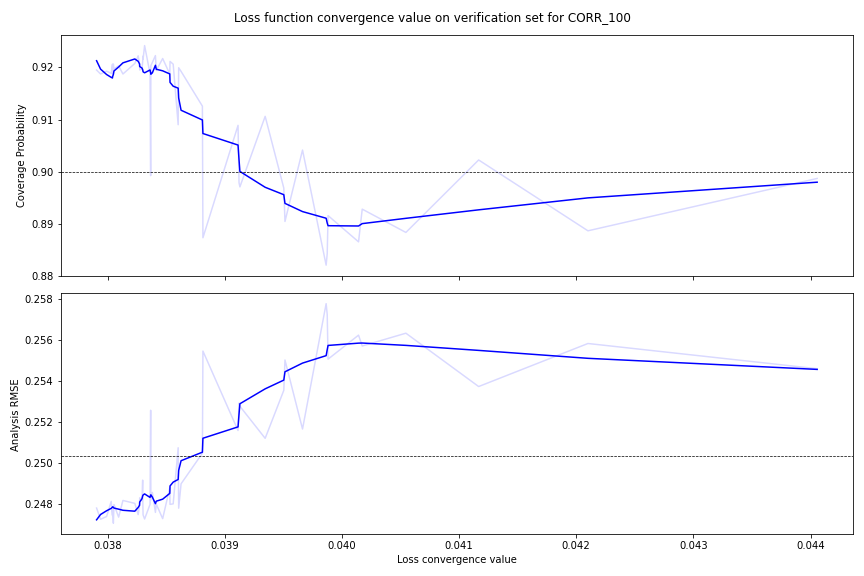
\includegraphics[width=.49\textwidth]{images/tmp/Convergence_CORR_100.png}
        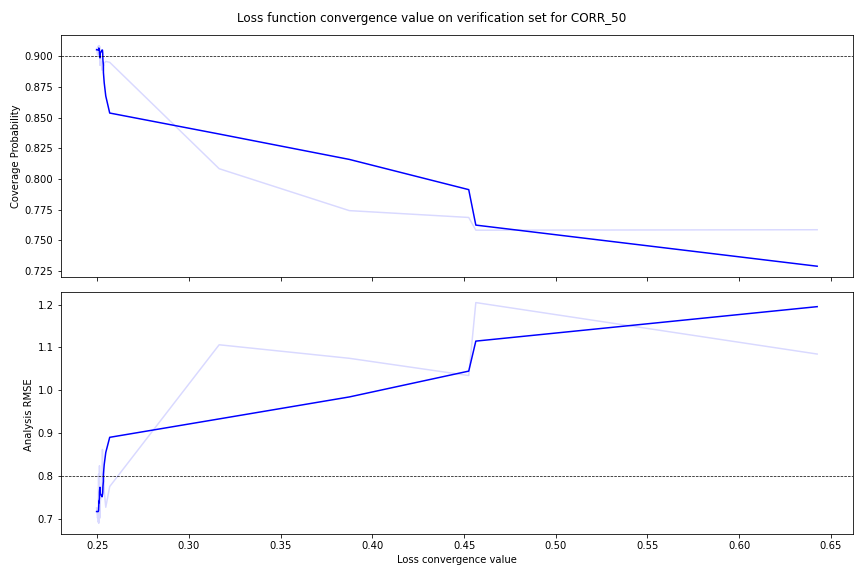
\includegraphics[width=.49\textwidth]{images/tmp/Convergence_CORR_50.png}
\end{figure}
\begin{figure}[hbt!]
    \centering
        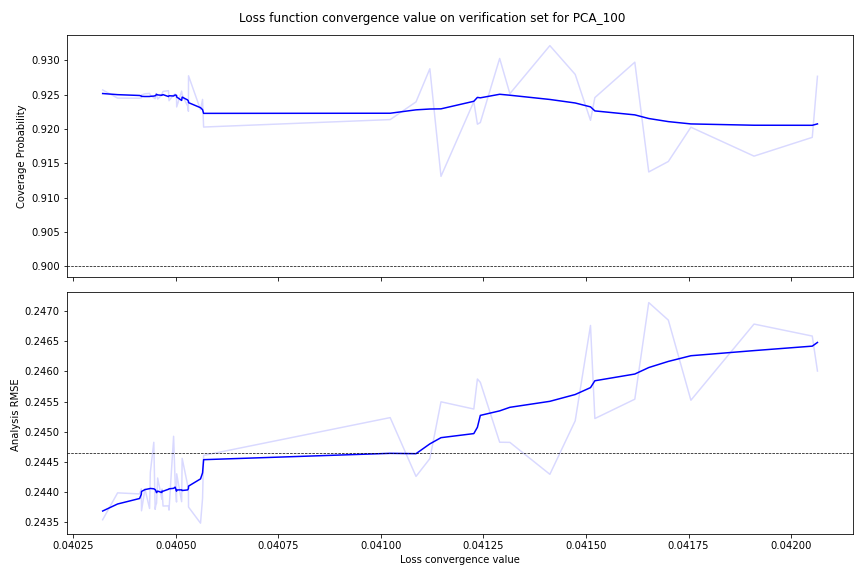
\includegraphics[width=.49\textwidth]{images/tmp/Convergence_PCA_100.png}
        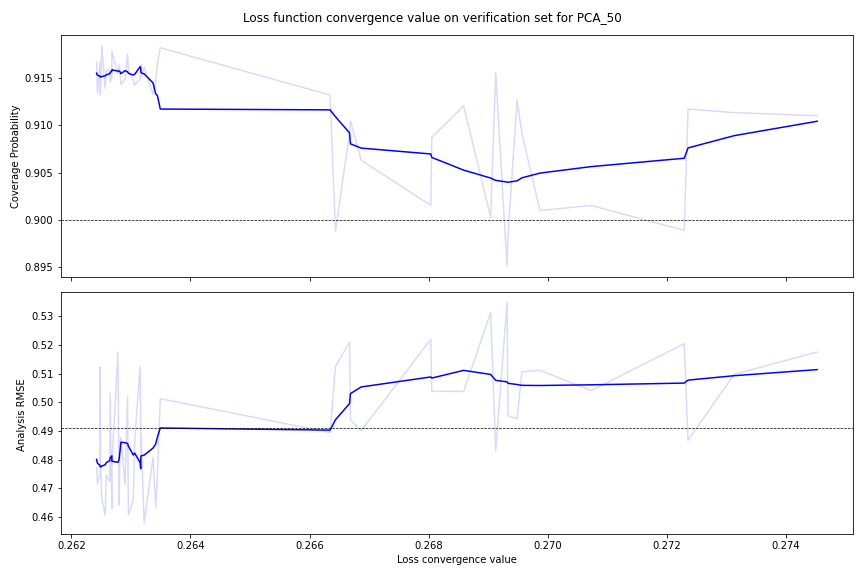
\includegraphics[width=.49\textwidth]{images/tmp/Convergence_PCA_50.png}
\end{figure}
\begin{figure}[hbt!]
    \centering
        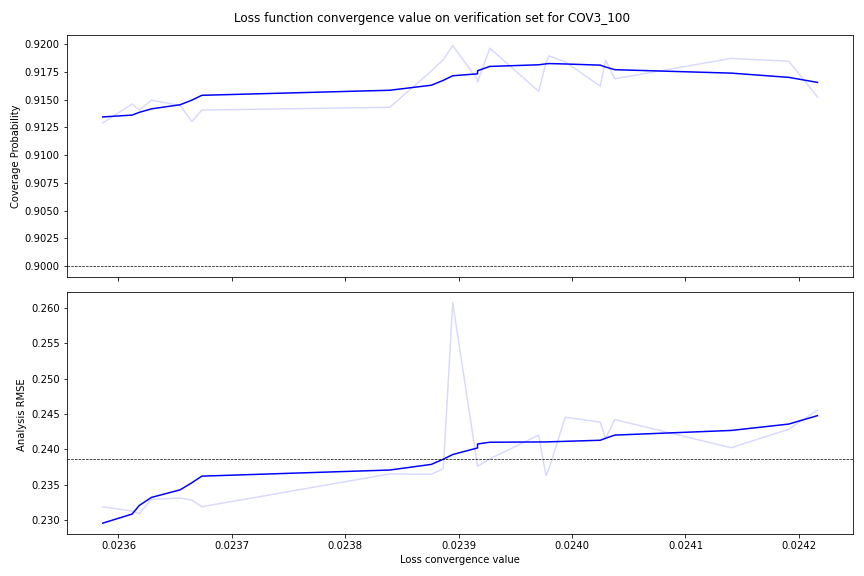
\includegraphics[width=.49\textwidth]{images/tmp/Convergence_COV3_100.png}
        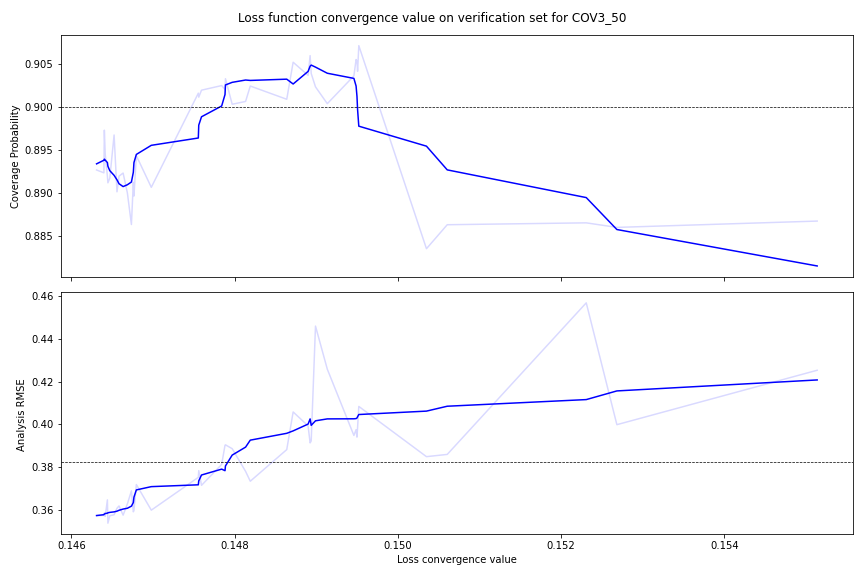
\includegraphics[width=.49\textwidth]{images/tmp/Convergence_COV3_50.png}
\end{figure}


Quantifying forecast uncertainty is a key aspect of data assimilation (DA) systems. In particular most DA methods rely on an accurate estimation of the probability density function (PDF) of the forecast errors or at least its covariance matrix (which suffices to describe the PDF under the assumption that errors are unbiased and Gaussian).

%In the process of data assimilation, it is of paramount importance to have a precise prediction covariance which represents the uncertainty of the forecast state. 

Data assimilation approaches such as optimal interpolation (OI, \cite{someoneXXXX}) or 3-dimensional variational methods (3DVar, \citep{parishandderber92}), assumes that the forecast error covariance matrix is independent of the sate of the system. Currently methods that provide an implicit (e.g. 4DVAR, \cite{bannister2016}) or explicit (e.g. EnKF \cite{houtekamerzhang2016}, PF \cite{vanLeewuenetal2019}) or hybrid \cite{bannister2016}, estimation of the state dependent forecast error PDF produce a remarkably improvement of the accuracy in the inference of the state and the forecast skill \citep{kalnay2003,carrassi2018}. However these improvements came at the cost of a significant increase in the computational cost with respect to methods in which the state dependence of the forecast error covariance is not taken into account. Moreover, even when state dependent covariances are estimated, an accurate representation of the contribution of model errors to the covariance is challenging \citep{tandeoetal2020}. 

%3DVar is a  classical assimilation technique (Fig. \ref{fig:ASdet}) that uses a fixed state-independent covariance, estimated using climatological forecast information. 
%And This approach is very very cheap computationally, but we do not have state-dependent covariance.

%\begin{figure}[hbt!]
%    \centering
%        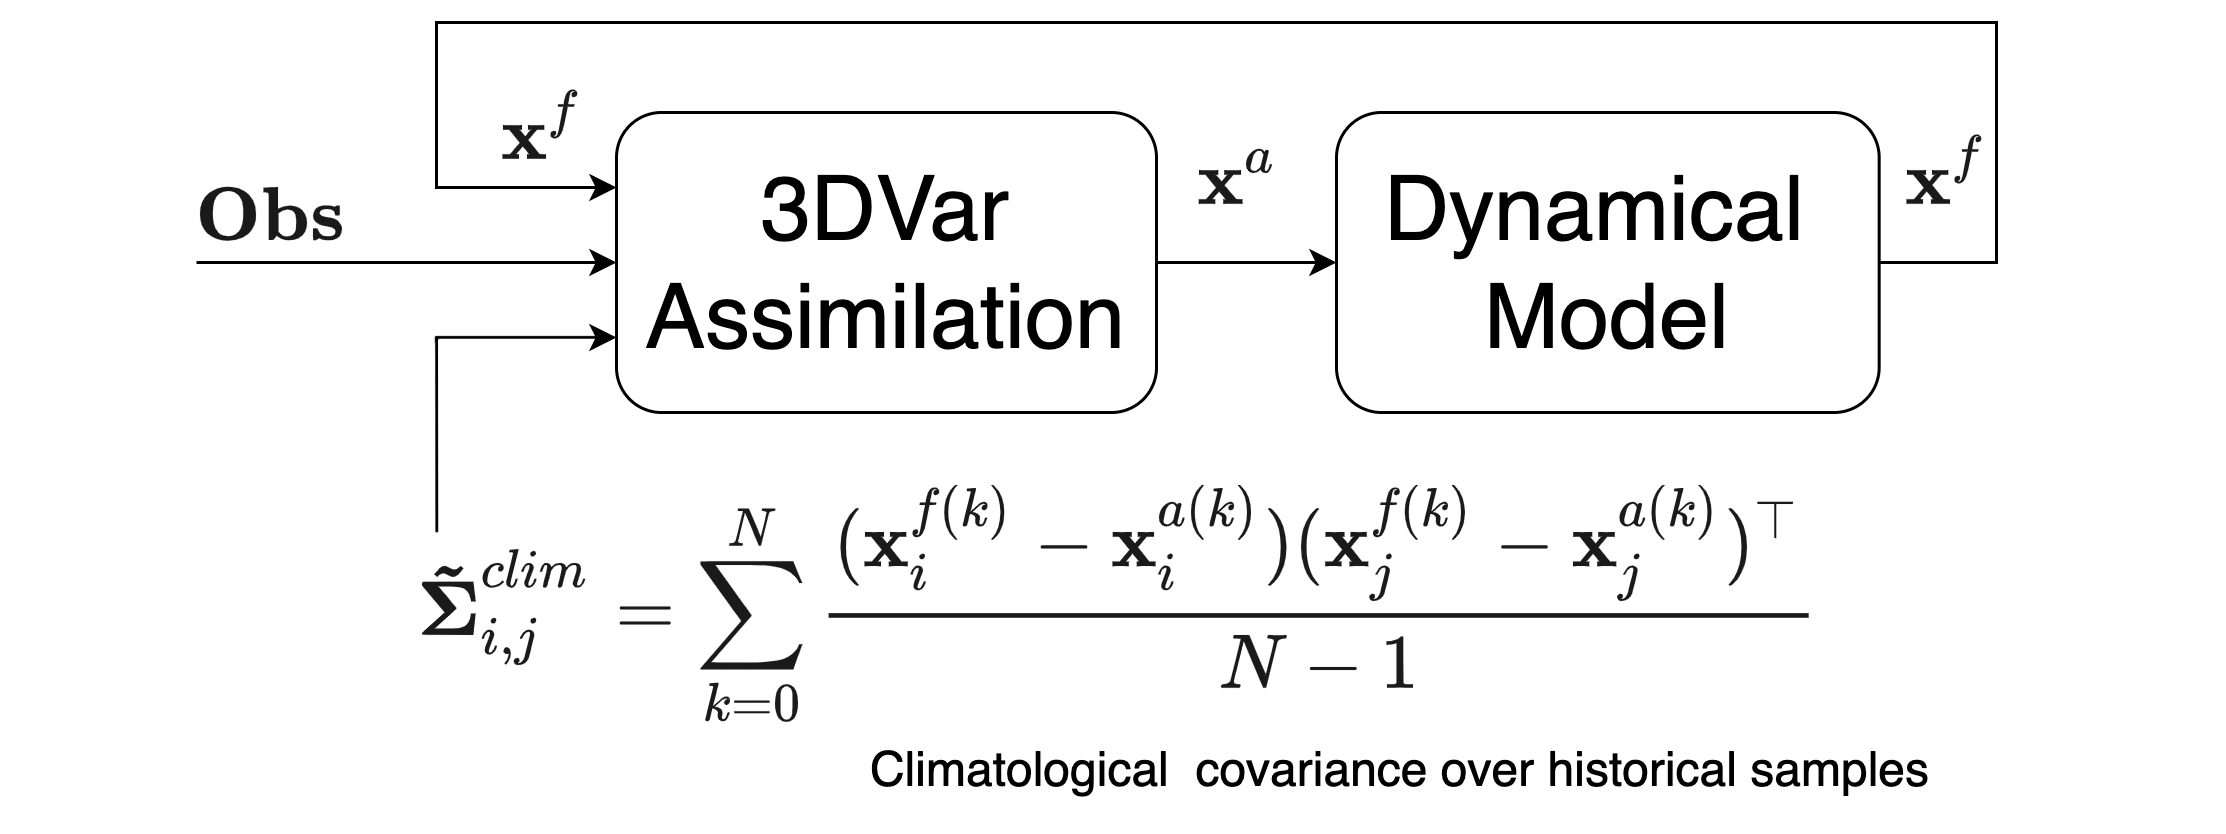
\includegraphics[width=.5\textwidth]{images/AsimDET.png}
%    \caption{caption}
%    \label{fig:ASdet}
%\end{figure}

%In the ensemble technique (Fig. \ref{fig:ASens}),  sigma  is estimated as the sample covariance of the forecast ensemble 
%This provides us with a state-dependent estimate of the prediction error.
%Some  important shortcomings in ensemble-based DA are the subestimation of variances due to sampling error, and the high computational cost

%\begin{figure}[hbt!]
%    \centering
%        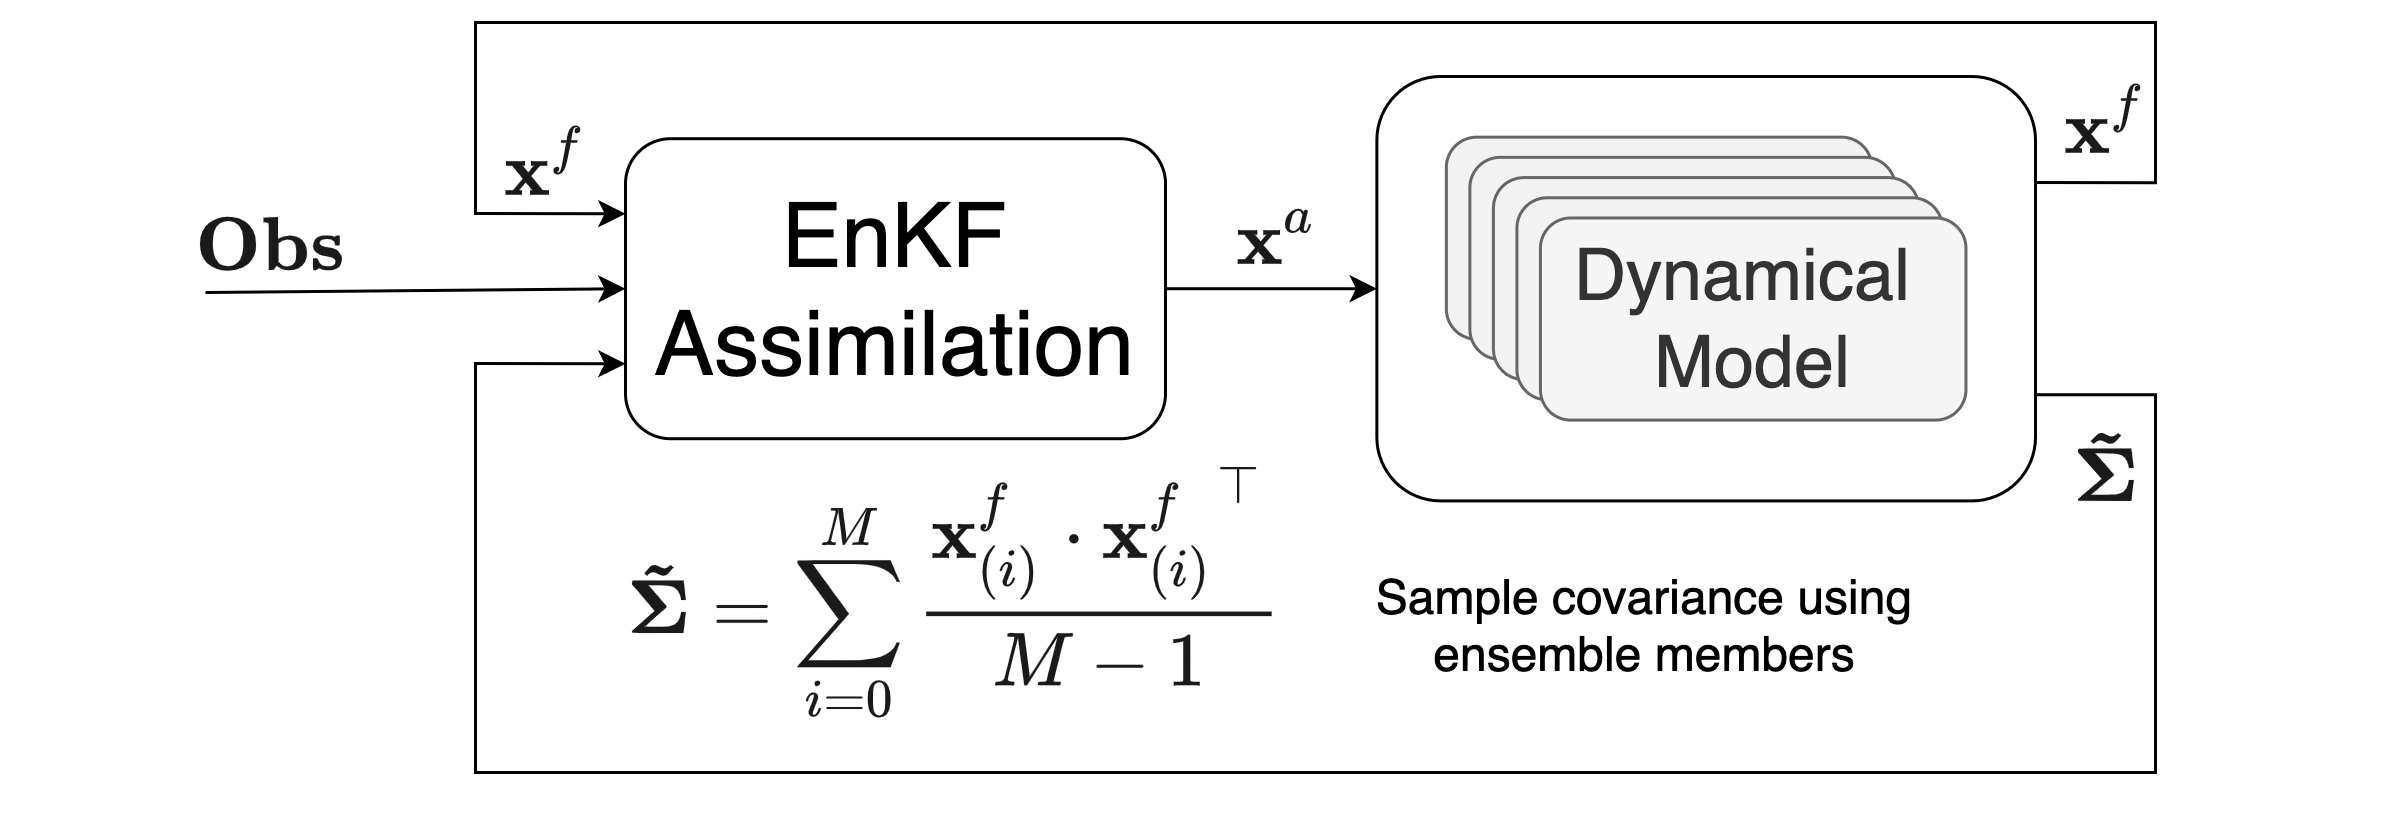
\includegraphics[width=.5\textwidth]{images/AsimENS.png}
%    \caption{caption}
%    \label{fig:ASens}
%\end{figure}

Recently machine learning methods have emerged as a promising way to estimate the forecast uncertainty (e.g. \citep{camporeale2,wang,gronquist2019,grooms2021,lguensat2018,saccoetal2022,irrgangetal2020}, among others). These methods provide an accurate estimation of the forecast uncertainty at a relatively low computational cost (i.e without the need to run the numerical model several or to run the adjoint of the numerical model). Moreover, some of these methods provide a way to estimate the uncertainty associated with model errors which are difficult to handle in state-of-the-art approaches (e.g. \cite{camporeale1,wang,saccoetal2021}). This is achieved by the use of uncertainty-aware loss functions allowing the ML algorithms to learn the errors statistics directly from the data. 

Most of these papers focused on the estimation of the forecast error variance (e.g. \cite{wang,camporeale1,gronquist2019,irrgangetal2020,saccoetal2022} among others). However for data assimilation the estimation of the full error covariance structure is fundamental. \cite{grooms2021} estimated the full covariance structure based on a machine learning method designed to provide an ensemble of perturbations of the state variables that represents possible realizations of the forecast error. This approach emulates the one used in ensemble forecasting but without the need to run the expensive numerical model to generate the ensemble members. \cite{lguensat2018} replace the numerical model for a surrogate model based on a local linear analog regression, thus significantly reducing the computational cost associated with the numerical integration of the ensemble. 

The estimation of a full error covariance matrix from data has been investigated in other contexts. \cite{Liuetal2018} implemented a deep learning model for the inference of the observation error covariance matrix and applied to position estimation for navigation applications. 
.... (Manuel: vos nos habias pasado varios papers sobre estimacion de covarianza con ML con otras aplicaciones que estaban muy interesante, creo que estaria bueno mencionarlos aca).


Relatively few papers investigated how these approaches can be coupled in a DA system. Few experiments has been conducted to address how machine-learning based forecast uncertainty estimation impact the quality of the estimated estate of a system, particularly when several assimilation cycles are performed. Also, as discussed in \cite{saccoetal2022}, short-lead time forecast uncertainty estimation, which is the most important lead time for DA, can be challenging. %How variance estimation biases that may arise in machine learning based uncertainty estimation can affect the accuracy of the analysis?

There are in the literature other approaches aiming to combine machine-learning and data assimilation. The similarities between DA and ML and their potential synergism has been introduced in \cite{hesiehandtang1998}.  \cite{farchietal2021,farchietal2022,boquetetal2019,brajardetal2020} proposed a framework in which machine learning is used for the estimation of the system dynamics and to represent model errors, while data assimilation provides an online continuous optimization of the data-driven model. Along the same line, \cite{brajard2021, farchietal2021b}, use a data assimilation approach to online training a machine learning based parametrization of the effect of unresolved scale dynamics within a numerical model. 
Other approaches aimed to a replacement of the full DA system by a neural network as in \cite{Harteretal2008}. In this approach the authors train a neural network that learns, from a given DA system, the magnitude and spatial patters of the state update introduced by the observations. 
\cite{buizzaetal2021} introduced the name "Data Learning" to describe several examples in which ML and DA can be combined to overcome their mutual weaknesses. These applications include: parameter estimation ..... 

In this work we extend the uncertainty quantification approaches discussed in \cite{saccoetal2022} for the estimation of the state-dependent full covariance matrix of a chaotic system and couple this estimation with a data assimilation system. We investigate three different approaches to estimate the full covariance matrix, one based on a direct estimation and the other two based on a dimension reduction approach. The methods proposed in this paper are flexible in the sense that they can be used to assimilate any kind of observations, even though those not available during the training period.   

This paper is structured as follows: Section \ref{SEC:METH} describes the different approaches for the estimation of the forecast error covariance including a brief review of the ensemble Kalman filter and the experimental settings. Section \ref{SEC:RES} analyzes the results obtained, and \ref{SEC:CONC} presents the main conclusions of this work as well as a discussion of future perspectives.

Otro paper de los primeros que parece pertinente para citar (mas en la linea de estimacion de modelo / parametrizaciones ) pero no logre descular exactamente que hacian. 


\section{Methodology}


\subsection{Sequential data assimilation}

In a sequential data assimilation cycle we aim to estimate the state of a dynamical system at regular time intervals by combining the information provided by a surrogate numerical model and a set of partial and noisy observations \citep{carrassi2018}.
We start by considering a chaotic dynamical system represented via the following Markov process
\begin{equation}
\label{EQU:sdm1}
\v x_{k} = \mathcal{M}_{k:k-1}(\v x_{k-1})+\gv \delta_k,
\end{equation}
where $\v x_{k}$ is an $M$-dimensional vector representing the state of the system at time $k$, $\mathcal{M}_{k:k-1}$ is a known surrogate nonlinear and chaotic model of the system dynamics that maps the state at time $k-1$ into time $k$. $\gv\delta_k$ represents the discrepancy $x_{k}$ and $\mathcal{M}_{k:k-1}(\v x_{k-1})$ due to the model imperfection (i.e. the model error). In this work we assume that the model error is a random variable sampled from an unknown probability distribution. Moreover, this distribution have a non-zero mean due to the presence of systematic model biases.   

Given a pointwise estimation of the state of the system at time $k-1$ ($\v x^a_{k-1}$) a forecast of the state at a time $k$ ($\v x^{f}_{k}$) can be obtained by integrating the dynamical model as in

\begin{equation}
\label{EQU:detfor}
\v x^{f}_{k} =  %\mathcal{M}_{k+l:k}(\v x^{d}_{0,k}),
\mathcal{M}_{k:k-1}(\v x^{a}_{k-1}),
\end{equation}
Note that forecast for longer lead times can be obtained by a recursive application of the numerical model. 
Then forecast error can then be defined as:  
\begin{equation}
\label{EQU:forerr}
\gv \epsilon_{k}^{f} = \v x^{t}_{k} - \v x^{f}_{k},
\end{equation}
where $\v x^{t}_{k}$ is the true state of the system at time $k$. Forecast errors are the consequence of an imperfect estimation of the state of the system at time $k$ and model errors. The magnitude and structure of both contributions to the forecast error are highly state dependent, meaning that the structure and magnitude of the component of the forecast error covariance matrix at time $k$ ($\gv P^{f}_{k} = [\epsilon_{k}^{f} {\epsilon_{k}^{f}}^T]$) are a function of the state. Data assimilation methods rely on the assumption that these errors are zero-mean, which is not usually the case. 

The state of the system is related to the observable quantities through the following observation equation:
\begin{equation}
\label{EQU:obsmodel}
\gv y_{k} = \mathcal{H}( \v x^{t}_{k} ) + \gv \nu_{k},
\end{equation}
where $\gv y_{k}$ is the M-dimensional vector containing the observable quantities, $\mathcal{H}$ is the observation operator (i.e. the function mapping state variables to the observable quantities) and $\gv \nu_k$ is the observation error which is assumed to be drawn from a Gaussian distribution with zero-mean and known covariance denoted $R_k$.

Given the forecast ($x^{f}_{k}$) and a set of observations ($y_{k}$) and assuming that their errors are unbiased (their mean is zero), the linear estimator that minimize the root mean square error with respect to the true state of the system is given by:

\begin{equation}
\label{EQU:analysis}
\begin{split}
&\gv x^a_{k} = x^f_{k} + \gv{K}\gv{H}^T(y_k - \mathcal{H}(x^f_{k}) ), \\
&\gv{K} = \gv{P}^f_k \gv{H}^T(\gv{H} \gv{P}^f_k \gv{H}^T + R_k)^{-1}, 
\end{split}
\end{equation}
where $x^a_{k}$ is the estimation of the system state (a.k.a the analysis) at time $k$, $\gv{H}$ is the tangent linear of the observation operator and $\gv K$ is the Kalman gain matrix which projects and filters the discrepancy between the observations and the forecasted observed quantities into the state space. This estimate of the state is also the maximum likelihood estimation of the state of the system under the assumption that the PDFs of the forecast errors and observation errors are both zero mean and Gaussian \citep{carrassi2018}. 


Once an estimation of the system state is obtained at time $k$, Equation \ref{EQU:detfor} can be used to forecast the state of the system for the next time, and the cycle can be repeated when a new set of observations became available. The accuracy of the estimate depends strongly on the ... P R ... 

In this work we develop methods to estimate the state-dependent error covariance matrix using machine learning approaches in the context of a data assimilation system. For completeness we first briefly describe the EnKF which is one of the most broadly used methods to incorporate the state-dependence of the forecast error covariance matrix in data assimilation applications for numerical weather prediction. In this paper, the EnKF is also used in the training of the machine learning algorithms and for their evaluation.

\subsection{EnKF}

The ensemble Kalman filter consists of a family of methods to optimally estimate the states of a dynamical system at several times from a set of noisy observations. The state of the system at time $k$, is obtained from a combination of a forecast of the system and a set of partial and noisy observations valid at that same time. To optimally combine the information provided by the forecast and the observations the EnKF relies on an estimation of the forecast error covariance matrix ($\gv P^{f}_{k}$) and of the observation error covariance matrix ($\gv R_k$).

$\gv P^{f}_{k}$ is estimated using a montecarlo approach in which we start assuming that we have a sample of states drawn from the estimated probability distribution of the state at time $k$ ($x^{a,(n)_{k-1}}$ for $n in 1 ... N$ with $N$ the sample size. The PDF of the forecast at time $k$ can be estimated by a sample resulting from the evolution of the individual ensemble members from time $k-1$ to time $k$ through the non-linear model equations:

\begin{align}
  \label{EQU:MODEL1}
  \v x^{f,(n)}_{k} =  \mathcal{M}^{(n)}_{k:k-1}(\v x^{a,(n)}_{k-1}) + \hat{\gv\delta}^{(n)}_{k},
\end{align}
where $x^{f,(n)}_{k}$ are the evolved ensemble members and $\hat{\gv\delta}^{(n)}_{k}$ represents the effect of model errors. 
The forecast ensemble mean at time $k$, $\overline{\v x}^{f}_{k} = \frac{1}{N} \sum_{n=1}^{N} \v x^{f,(n)}_{k}$ provides a pointwise estimation of the state. 
Along this lines $\gv P^{f}_{k}$ can be estimated from the forecast sample:

\begin{equation}
\label{EQU:SIGMA}
\gv P^{f}_{k} = \frac{1}{(N-1)}\sum_{n=1}^{N} \left(\v x^{f,(n)}_{k}-\overline{\v x}^{f}_{k}\right)\left(\v x^{f,(n)}_{k}-\overline{\v x}^{f}_{k}\right)^\top .
\end{equation}


\subsection{Machine learning covariance estimation}

\subsubsection{Machine learning based estimation of the forecast uncertainty}

Aca describimos como estimar la varianza de un forecast usando ML con la funcion de costo RMSE-EXT. 

A continuacion se describen las extensiones de esta metodologia para estimar la matriz de covarianza.

\subsubsection{Time-independent correlation method}

Asumiendo que la matriz de correlacion es constante e igual a la climatologica

\subsubsection{Time-independent correlation in the PCA space mehtod}

Asumiendo que la matriz de correlacion es constante e igual a la climatologica pero en el espacio de las PCAs.

\subsubsection{Direct estimation of the state dependent covariance}

No asumiendo nada de lo anterior y extendiendo la funcion de costo RMSE-EXT a las covarianzas. 

\subsection{Coupling with data assimilation}

Aca explicamos como acoplar la estimacion de la incertidumbre con ML con DA.


%We propose to use a neural network to estimate the covariance needed for data assimilation. 

%\begin{figure}[hbt!]
%    \centering
%        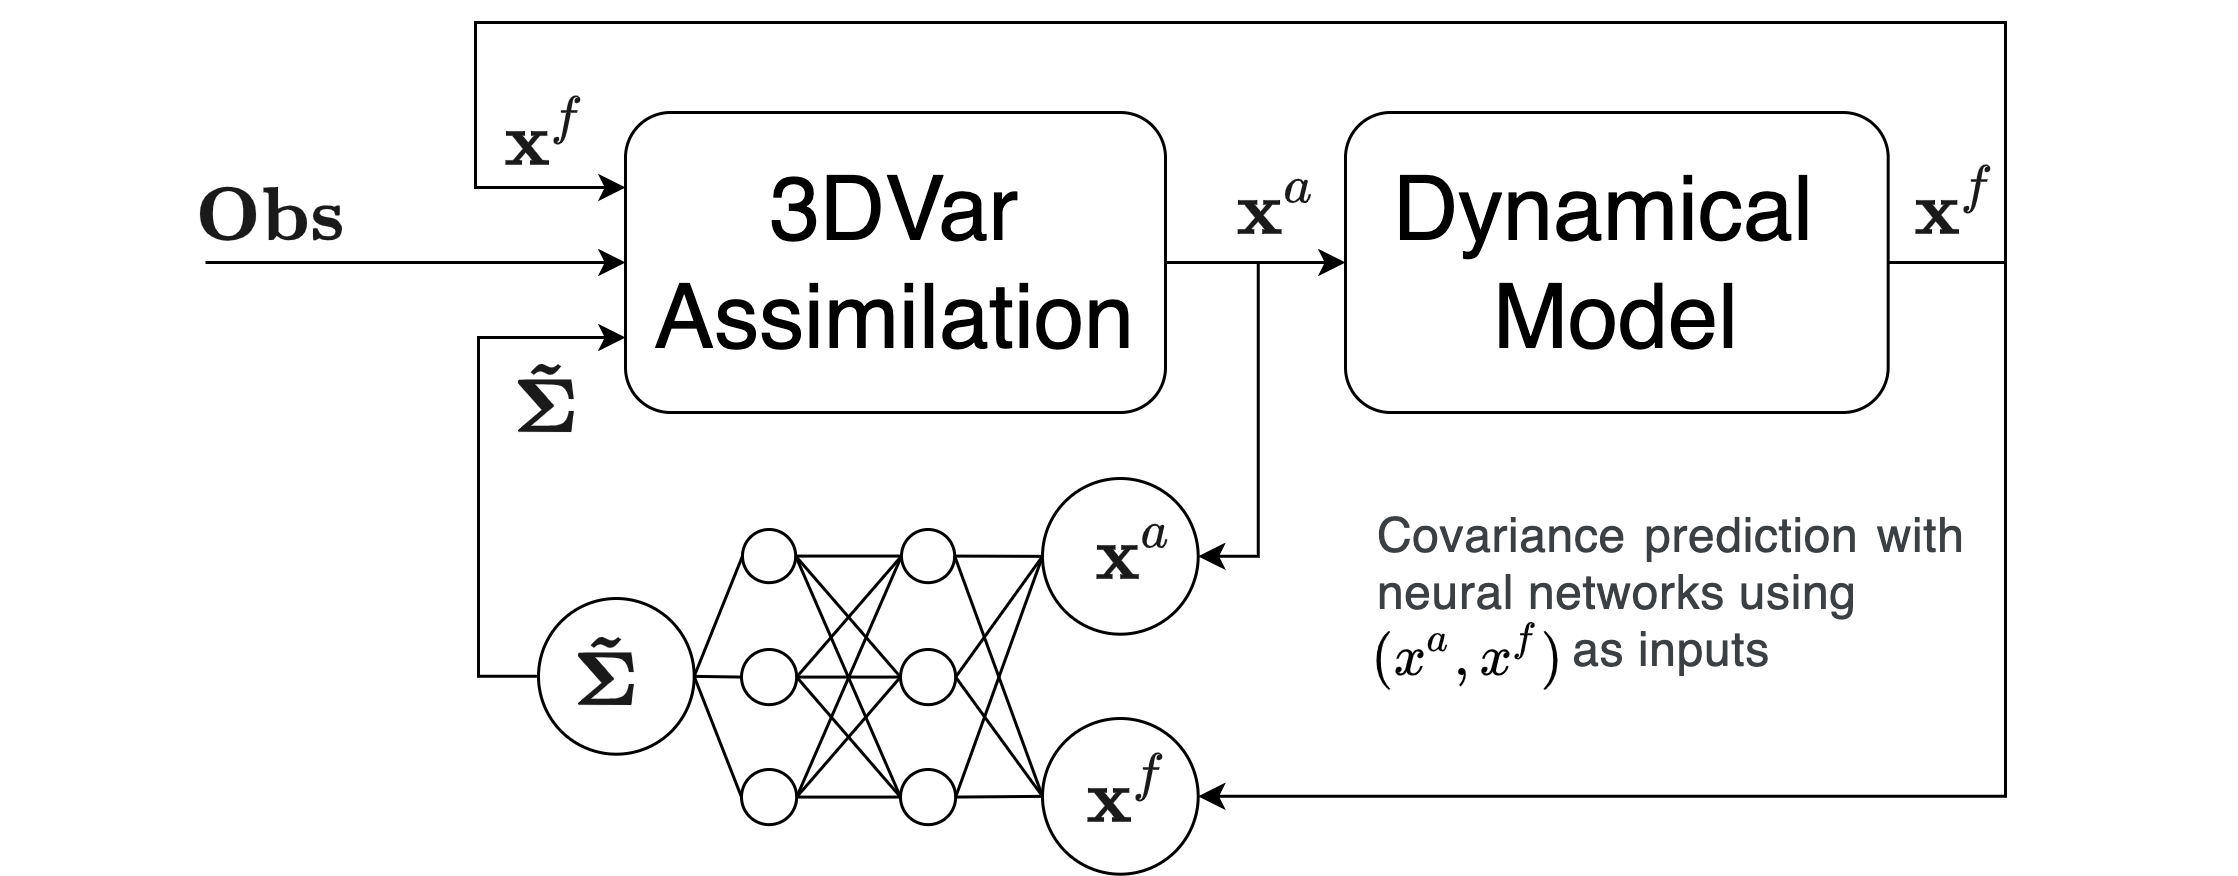
\includegraphics[width=.5\textwidth]{images/AsimNET.png}
%    \caption{caption}
%    \label{fig:ASnet}
%\end{figure}

%In fact we are going to feed the neural network with: the forecast at the desired lead time and its initial conditions (as shown in fig. \ref{fig:ASnet}) to estimate the error covariances, to conduct a new assimilation cycle, to generate a new analysis and go on.

%And we want to train this network without explicitly using information from the ensembles.

%Then we need to use a loss function that is sensitive to the forecast error.  
%For example Wang uses a loss function based on the observation likelihood assuming a Gaussian distribution 

%while Camporeale relies on CRPS and Brier score to achieve this. 

%We are going to use a loss function based on a local error estimate in a kind of semi-supervised training in three differents ways

\subsection{Experimental design}

\subsubsection{Numerical model}

Breve descripcion del modelo (en este caso seria solo escenario modelo imperfecto).

\subsubsection{Network architecture and training}


\begin{figure}[hbt!]
\centering
        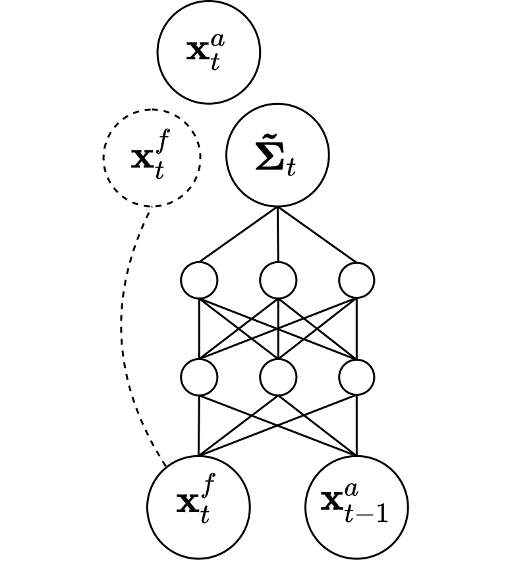
\includegraphics[width=.25\textwidth]{images/trainNET.png}
        \caption{The neural network is train to estimate the error present in the forecast used as input and the analysis given as target}
\label{FIG:TRAINNET}
\end{figure}

Descripcion de la arquitectura utilizada y como se entrenan las redes


\subsubsection{Baseline experiments}

Aca va la lista de experimentos a realizar (pero sin subsecciones para cada uno ya que todos los detalles estan explicados antes. Aca es solo decir que combina cada experimento y una motivacion. 

%\subsubsection{3DVar}

%A time independent covariance matrix using 3DVar technique. 

%\subsubsection{ENS50}

%A classic EnKF approach using 50 ensemble members. $\Sigma$ is estimated as the sample covariance of the forecast ensemble.

%\subsubsection{ENS5}

%A classic EnKF approach using 5 ensemble members. $\Sigma$ is estimated as the sample covariance of the forecast ensemble.

%\subsection{ANN-based variance estimation}

%\subsubsection{ANN}

%A neural network is used to estimate the variance terms (main diagonal of Pf). Off diagonal terms are estimated assuming a time-independent error correlation matrix. The network also provide a correction for the forecast systematic errors. The input to the network is a deterministic forecast. 

%\subsubsection{ANN-PCA}

%A neural network is used to estimate the covariance matrix in a base defined by the eigenvectors of the climatological error covariance matrix. This is done in an attempt to estimate the evolution of the full covariance matrix in a reduced-dimension space. The input to the network is a deterministic forecast.

%\subsection{ANN-based covariance estimation}

%\subsection{Network architecture and training}
%Fully connected NN with 2 hidden layers. 
%Loss function is based on the likelihood of the targets (analysis) conditioned on the input of the network (short range deterministic forecasts), this allows us to simultaneously estimate a correction for the forecast biases and the forecast uncertainty. 
%Networks are trained using a large dataset of short-range deterministic forecasts and their corresponding analysis obtained with a 50 member LETKF assimilation cycle. The model used to generate the analysis is an imperfect model (with respect to the model used to generate the observations).  

%\subsection{DA Experiments}
%Data assimilation experiments are conducted using these 4 methods to provide a first-guess and its associated uncertainty. The system is partially observed (one observation every other grid point). The same imperfect model used to generate the training sample is used in the different data assimilation experiments. Validation is always performed against the nature run. 

%\section{Experiment Design}

%What is really important about this slide is that we use the two-scale Lorenz96 model to generate a truth run. 
%Then, we generate the observations set by adding noise to  the state in the truth set.
%we use the one-scale Lorenz96 model to generate the forecasts simulating an imperfect model.
%Then, with the forecasts model and observations set we generate analyses using the ensemble kalman filter.
%Now With the analyses and forecasts, we generate the dataset that will be used to train the neural networks. 
%The state is 50\% observed, meaning that there are state variables that are never observed and we used multilayer perceptrons with two hidden layers.



\section{Results}

\begin{figure}[hbt!]
        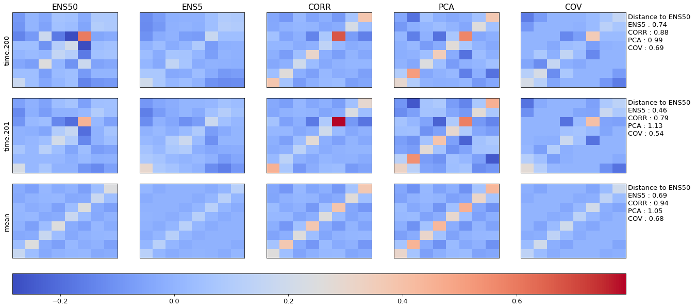
\includegraphics[width=\textwidth]{images/CovMX.png}
        \caption{Each column represent the covariance matrix estimated by each methods. The first and second rows correspond to two consecutive times, while the third row shows the mean covariance matrix over all the testing set. The table on the right  shows the frobenius distance between each method with the ensemble of 50 members}
\label{FIG:COVMXS}
\end{figure}

Figures \ref{FIG:COVMXS} shows the covariance matrices estimated by each method. 

The first and second row are snapshots of the point estimates covariance for two consecutive times while the third row is the mean over all the testing dataset.

On the right of the figure, it is shown the frobenius distance of each method with the 50-member ensemble.

With this figure we want to compare the structure of the covariance matrix estimated by each method
With the  ensemble as a reference.

For example, Corr and PCA experiments do not seem to preserve much of the structure of the 50-member ensemble . . . except for some maxima on the main diagonal that are correctly identified.  Also both methods have the large distance values,  with PCA being the largest.

For the COV experiment, even though it estimates a band matrix and its fourth and fifth diagonal are fixed at zero, the structure of the 50-member ensemble is recognizable 

\begin{figure}[hbt!]
        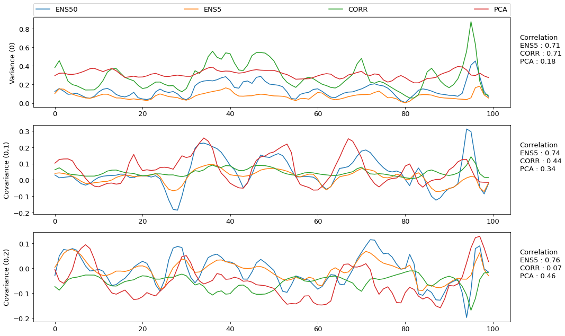
\includegraphics[width=\textwidth]{images/evolObsPCA.png}
        \caption{Time evolution over 100 consecutive time steps of the variance (top), the first and second covariance (middle and bottom plot respectively) of an observed variable for each estimation methods. The table on the right of each plot shows the correlation coefficient of each methods with an ensemble of 50 members }
\label{FIG:EVOLOBSPCA}
\end{figure}

The figure \ref{FIG:EVOLOBSPCA} shows the time evolution over 100 cycles of assimilation of only one state variable. In this case, an observed variable. 

The figure on top shows the evolution of the variance for each experiment. The figure in the middle, shows the value for the first covariance 
And the bottom figure, the value of  the second convariance

On the right of every figure  are the correlation coefficient of each method with the 50-member ensemble.

Something  notable about the figure on top is how PCA (red line) shows very little variability as opposed to CORR (green line) which seems to follow the ensemble pretty well.  

And also how this behavior is reversed in  the plot at the middle.

And if we look at the bottom figure, the corr experiments is completely uncorrelated.

\begin{figure}[hbt!]
        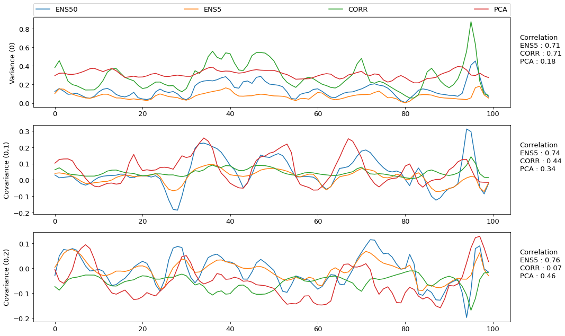
\includegraphics[width=\textwidth]{images/evolObsPCA.png}
        \caption{Same as figure \ref{FIG:EVOLOBSPCA} but on a not observed variable.}
\label{FIG:EVOLNOBSPCA}
\end{figure}
It is interesting to distinguish between observed and unobserved variables because the assimilation methods do not have observation  to correct them so that  the impact of estimated covariances in the resulting analysis is huge.

And it is remarkable how PCA performs in this case (fig. \ref{FIG:EVOLNOBSPCA}). 
Look at the amplitude of the variance compared to the observed variable where it was almost flat. 

And this makes sense because the PCA network learns the uncertainty in a space aligned with the maximum error variability, so it manages to focus where the uncertainty is largest.

\begin{figure}[hbt!]
        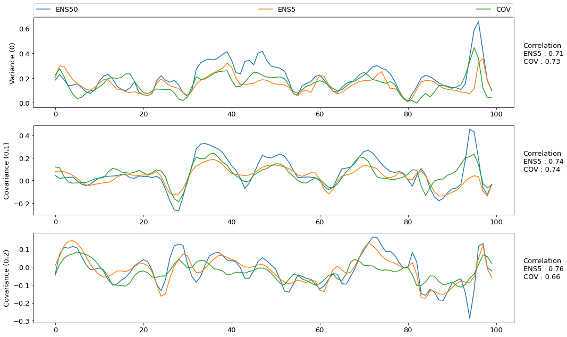
\includegraphics[width=\textwidth]{images/evolObsCOV.png}
        \caption{Same as figure \ref{FIG:EVOLOBSPCA} but comparing only the COV experiment with both ensemble (50 a 5 members)}
\label{FIG:EVOLOBSCOV}
\end{figure}

The COV network has more degree of freedom compared to the previous ones. The performance of this method is notably better for both variances and covariances (see figure \ref{FIG:EVOLOBSCOV})as it follows very closely the time evolution of the 50 member ensemble.

Indeed the time correlation coefficient is about 70\% in all the estimated parameters.  

\begin{figure}[hbt!]
        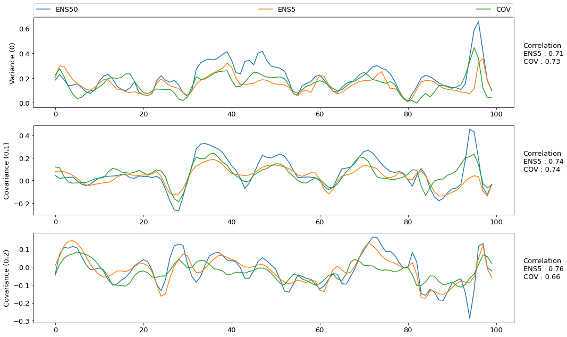
\includegraphics[width=\textwidth]{images/evolObsCOV.png}
        \caption{Same as figure \ref{FIG:EVOLOBSCOV} but for a not observed variable }
\label{FIG:EVOLNOBSCOV}
\end{figure}

and the same is true for unobserved variables (Fig. \ref{FIG:EVOLNOBSCOV}). 

The NN appears to capture a large part of the time variability of variances and covariances. 

Note the high-correlation coefficients again!!!

but so far we have made a qualitative analysis of the covariance obtained with each method, 
but we are interested in knowing  the performance of each method in a long assimilation cycle.

\begin{figure}[hbt!]
        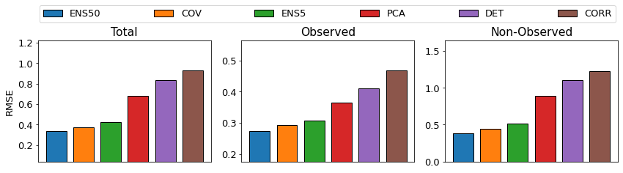
\includegraphics[width=\textwidth]{images/perfoComp.png}
        \caption{Covariance Matrices}
\label{FIG:COMPPERF}
\end{figure}

The figure \ref{FIG:COMPPERF} shows the total  error reach by each method over 10 thouthen cycles of assimilation 
and  also the error on observed and unobserved variables. 

For me, the biggest surprise was PCA, because in the qualitative analysis it was not doing very well. 
I think this is because PCA concentrated its predictive power where the error variability is higher due to lack of observations and, in particular,  where the assimilation method most needed it.

The error of the covariance method  is impressive. It managed to beat the small ensemble KF and it is even competitive with the 50member ensemble.


\section{Conclusion}
Results show that our approach can produce state-dependent estimations of the forecast uncertainty without the need of an ensemble of states (at a much lower computational cost),  particularly in the presence of model errors. This opens opportunities for the development of a new type of hybrid data assimilation systems combining the capabilities of machine learning and ensembles.
 
\begin{itemize}
    \item Training NNs with single forecasts! 
    \item ANN-based error covariance matrix prediction allows a stable data assimilation cycle.
    \item PCA and COV experiments clearly outperform 3DVAR.
    \item COV outperforms PCA and the small ensemble experiment.
    \item Relative performance of the different networks is mainly explained by their ability in capturing the state dependent structure of the error covariance
    \item High-dimensional states are a challenge. Parameterizations of the covariance are required.
\end{itemize}
 
For final conclusions we can mention that, we use neural networks to estimate the uncertainty from a deterministic forecast.

That the trained networks using the loss function based on local error estimation achieve a prediction that allows long assimilation cycles  . . . .  . .  improving the performance of the 3DVar method and at a much lower computational cost than the ensembles method. 

And this is because networks trained in this way manage to capture an important part of the structure of the state-dependent error covariance. 

and finally we leave as future work to analyze how these techniques can be extended to high dimensional problems.

 
\bibliography{references}
\end{document}
